
	Para realização efetiva do projeto proposto, as seguintes atividades se tornam essenciais:

	\begin{itemize}	
		\item \textbf{Metodologia de Desenvolvimento}

			Durante esta atividade, o responsável deverá ajustar uma Metodologia para Desenvolvimento do projeto, de forma que a mesma se adeque de forma simples ao Contexto em que estamos inseridos. Serão descritos, nessa atividade, como serão feitas as Pesquisas, Avaliações e Análise dos Resultados.

		\item \textbf{Fundamentação Teórica}

			Durante esta atividade, o responsável deverá obter a fundamentação teórica necessária para a realização do projeto proposto. Pesquisas bibliográficas sobre o contexto deverão ser realizadas com o objetivo de obter o máximo de material possível para apoio à equipe.

		\item \textbf{Planejamento das Avaliações a serem Realizadas}

			Durante esta atividade, o responsável (que será toda a equipe) deverá planejar as Avaliações que serão realizadas de forma que as mesmas possam obter o máximo de informações possível, garantindo assim, maior efetividade na Avaliação.

		\item \textbf{Desenvolvimento dos Questionários e Entrevistas}

			Durante esta atividade, o responsável (que será toda a equipe) deverá desenvolver Questionários e Entrevistas com base na Fundamentação Teórica e, principalmente com base nas 10 (dez) Heurísticas de Nielsen.

		\item \textbf{Aplicação dos Questionários e Entrevistas}

			Durante esta atividade, o responsável (que será toda a equipe) deverá aplicar os Questionários e Entrevistas com o máximo de usuários possível. Lembrando que a aplicação deverá ser feita levando em consideração a faixa social em que o Usuário está presente. Ou seja, a aplicação deve ser feita com jovens, adultos, idosos, conhecedores de TI, leigos em TI e etc.

		\item \textbf{Compilação e Análise dos Resultados}

			Durante esta atividade, o responsável (que será toda a equipe) deverá Analisar todos os dados obtidos através das Entrevistas, Questionários e Análise do \textit{ASES}, e com isso, conseguir obter uma conclusão sobre a Usabilidade do Sistema Enturma.

		\item \textbf{Divisão e Planejamento das Atividades de Adaptação}

			Durante esta atividade, o responsável deverá levantar as atividades necessárias para adaptação do sistema e alocar responsáveis para cada atividade.

		\item \textbf{Adaptação do Sistema}

			Durante esta atividade, o responsável (que será toda a equipe) deverá executar as atividades levantadas na atividade anterior, com o objetivo de adaptar o sistema, tornando-o mais simples e eficiente no uso.

		\item \textbf{Aplicação dos Questionários e Entrevistas}

			Durante esta atividade, o responsável (que será toda a equipe) deverá aplicar, novamente, todos os Questionários e Entrevistas aplicados anteriormente, com o objetivo de obter uma comparação dos resultados das Avaliações realizadas no sistema antigo e na nova versão do mesmo.

		\item \textbf{Compilação e Análise dos Resultados}

			Durante esta atividade, o responsável (que será toda a equipe) deverá compilar todos os dados obtidos durante todo o projeto, interpretar os mesmos e chegar a alguma conclusão referente a evolução da Usabilidade do Sistema Enturma.
	\end{itemize}

\subsection{Resumo da proposta}
	
	[Escrever um resumo da proposta de trabalho do grupo, responder o que será realizado, qual o ponto de partida e realizar conexões com a fundamentação teórica apresentada.]

\subsection{Estrutura Analítica do Projeto}
	
	[A Estrutura Analítica de Projetos (EAP), do Inglês, Work breakdown structure (WBS) é uma ferramenta de decomposição do trabalho do projeto em partes manejáveis. É estrutura em árvore, hierárquica (de mais geral para mais específica) orientada às entregas que precisam ser feitas para completar um projeto.

	O objetivo de uma WBS é identificar elementos terminais (os produtos, serviços e resultados a serem feitos em um projeto). Assim, a WBS serve como base para a maior parte do planejamento de projeto.
	
	A dica de ferramenta a ser utilizada para elaborar a EAP é o XMIND 
	
	http://www.xmind.net/ ]

\subsection{5.3. Lista de software}
	
	Durante o processo de Avaliação do Sistema Enturma, que engloba desde o Planejamento da Avaliação até a Análise dos Resultados obtidos, serão usados diversos \textit{softwares} e tecnologias para apoiar a Equipe, tais como:

	\begin{itemize}
		\item \textbf{Git}

			O sistema Git será utilizado para Gerência de Configuração e Controle de Versões durante o projeto.

		\item \textbf{GitHub}
			
			Será utilizado como repositório remoto do GIT, para compartilhamento dos dados entre a Equipe.

		\item \textbf{LaTeX}

			Será utilizado para o desenvolvimento de toda a documentação produzida durante a execução deste projeto.

		\item \textbf{Sublime}

			Será utilizado como IDE para o desenvolvimento da Documentação e durante a Evolução do sistema Enturma.

		\item \textbf{GITTER}

			Será utilzado para comunicação, via GitHub, da Equipe durante o Desenvolvimento Projeto.

		\item \textbf{ASES}

			Sistema desenvolvido pelo Governo Federal para Avaliação da Acessibilidade em Sistemas Web.

	\end{itemize}

\subsection{Cronograma de Atividades}

	O Cronograma do Projeto pode ser obtido acessando o link do Drive do Projeto. Como representação, segue a parte inicial do Cronograma de Atividades:

	\begin{figure}[H]
		\centering
		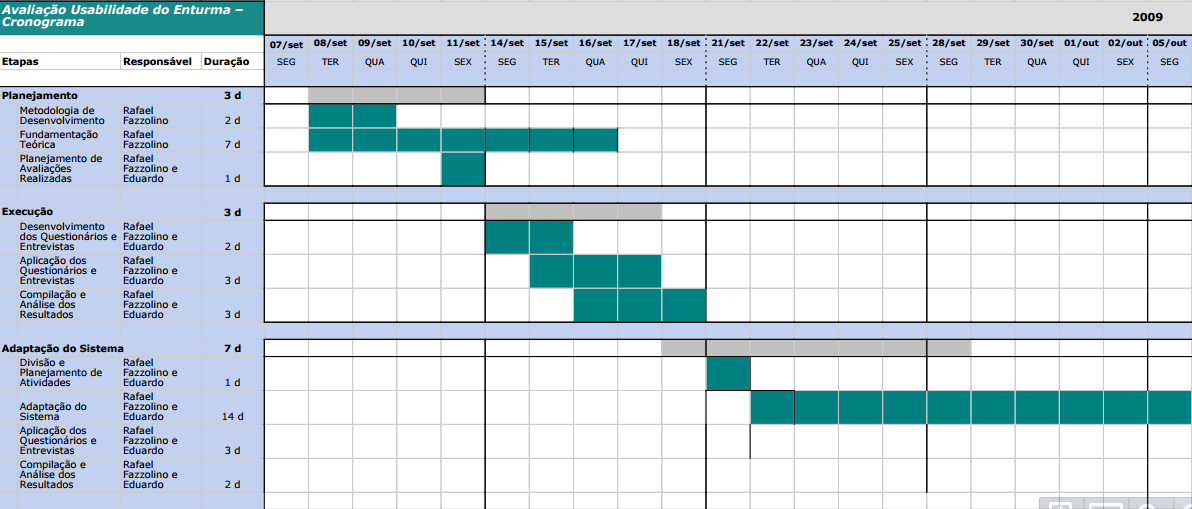
\includegraphics[width=1\textwidth]{imagens/cronograma}
		\caption{Cronograma Inicial do Projeto}
		\label{img:cronograma}
	\end{figure}

